% !TEX encoding = UTF-8 Unicode
\documentclass{scrartcl}
\usepackage{report}

\usepackage{fontspec}
\setmainhangulfont[Path=../fonts/,
  BoldFont={KoPub Batang Bold},
  ItalicFont={KoPub Dotum Light},
  BoldItalicFont={KoPub Dotum Bold}
]{KoPub Batang Light}
\setsanshangulfont[Path=../fonts/,
  BoldFont={KoPub Dotum Bold},
  ItalicFont={KoPub Batang Light},
  BoldItalicFont={KoPub Batang Bold}
]{KoPub Dotum Light}

\setkomafont{disposition}{\normalfont\bfseries}

% \cfoot{Page~\thepage~of~\pageref{LastPage}}

\begin{document}

\title{공간통계 보고서}
\subtitle{Burger Index: New city development index}
\author{이경원}
\affil{서울대학교 통계학과}
\date{\today}
\maketitle


\begin{abstract}
    본 보고서에서는 버거지수(Burger Index; BI)에 대해 알아보고, 이 값이 도시의 발전도를 나타낼 수 있는지에 대해 공간통계학의 관점에서 살펴보고자 한다. 
\end{abstract}

\section{Introduction}   

현재, 전 세계 인구의 절반 이상은 도시지역에 거주하고 있다. 도시의 발전도는 인구밀집도와 높은 상관관계가 있으며 인구가 많은 큰 도시를 뜻하는 대도시(metropolitan)\가 정치, 경제, 문화의 중심이 되는 도시를 일컫는 데 사용되기도 한다. 도시발전지수(city development index)는 도시의 발전도를 의미하는 지표로 문화, 경제 등 다중공산성(multicolinearity)이 적다고 판단되는 여러 항목을 바탕으로 계산할 수 있다. 

버거지수(Burger Index; $BI$)는 2014년 한 트위터 유저(\autoref{fig:firstbi})에 의해 제안된 개념으로 $B,~M,~K,~L$을 각각 특정 도시 내의 버거킹, 맥도날드, KFC, 롯데리아 지점 수라고 했을 때 다음과 같이 정의된다
\begin{equation}\label{eqn:originbi}
    BI = \frac{B+M+K}{L}.
\end{equation}
해당 유저는 버거지수가 도시발전지수로 사용될 수 있다고 주장하였으며, 이후에도 \citet{jang2014} 등에 의해 탐색적 자료분석을 통한 정성적 확인이나 \autoref{fig:jangmap}와 같은 위상구조를 이용한 시각화가 이루어졌다. 반면에 실제 지리정보시스템(geographic information system; GIS)을 이용한 시각화나 회귀분석을 통한 정량적 분석은 시도된 적이 거의 이루어지지 않았고, 버거지수의 구체적인 의미를 파악하는 데 어려움이 있었다.

\begin{figure}[!ht]
    \centering
    \begin{subfigure}[b]{0.6\textwidth}
        
\includegraphics[width=\textwidth]{../figs/burgerindex.jpeg}
        \caption{최초로 제안된 버거지수}\label{fig:firstbi}
    \end{subfigure}~
    \begin{subfigure}[b]{0.3\textwidth}
        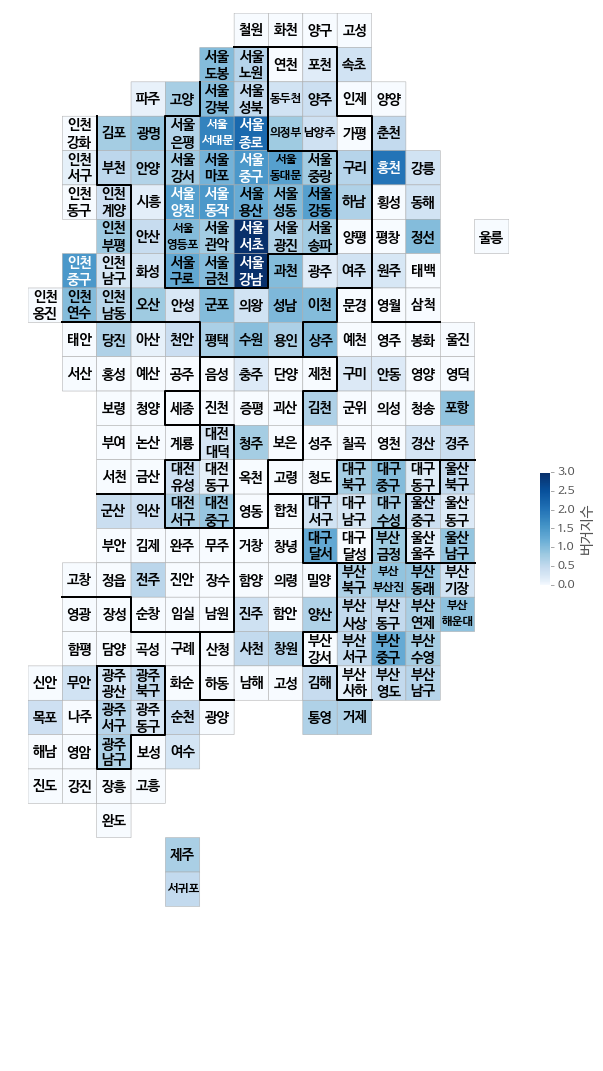
\includegraphics[width=\textwidth]{../figs/burgerindexmap.png}
        \caption{\citet{jang2014}, 버거지수 지도}\label{fig:jangmap}
    \end{subfigure}
    \caption{기존의 버거지수 관련 그림들}
\end{figure}

이번 보고서에서는 버거지수를 국내 지도에 시각화하고, 이 값이 실제로 도시발전지수에 사용될 수 있는지에 대해 살펴보고자 한다. \autoref{sec:data}에서는 자료 설명과 전처리 과정을, \autoref{sec:eda}에서는 전처리된 자료를 바탕으로 시각화 및 수치적 요약을 다룬다. \autoref{sec:sreg}에서는 공간회귀분석(spatial regression)\을 통해 버거지수가 실제로 어떤 의미를 가지고 있는지를 알아보고자 하며 그 결과와 논의를 각각 \autoref{sec:result}, \autoref{sec:con}에 정리하였다. 분석에 사용된 코드들은 github\footnote{\url{https://github.com/heleeos/BurgerIndex}}에 공개되어 있다.

\section{Data}\label{sec:data}

\subsection{Data Description}\label{subsec:data:desc}

\autoref{tbl:data:description}에 보고서에서 사용한 자료를 정리하였다. 

\begin{table}[ht]
    \centering
    \resizebox{0.8\textwidth}{!}{
	\begin{tabular}{c|p{13em}|c|c}
        \hline
        이름 & 설명 & 형태 & 출처 \\ \hline
		\texttt{burget/*} & 2019년 4월 기준 시군구별 패스트푸드 매장(버거킹, 맥도날드, KFC, 롯데리아, 맘스터치) 수 & xlsx(엑셀) & github\footnote{\url{https://github.com/idjoopal/BurgerIndex2019}} \\ \hline
		\texttt{pop/201903.xlsx} & 2019년 3월 기준 시군구별 주민등록 인구 자료 & xlsx(엑셀) & 국가통계포털\footnote{\url{http://kosis.kr/index/index.do}} \\ \hline
		\texttt{map/*} & 2019년 2월 기준 대한민국 시군구 단위 GIS 자료 & shp 등 & GIS DEVELOPER\footnote{\url{http://www.gisdeveloper.co.kr/?p=2332}} \\ \hline
    \end{tabular}
    }
	\caption{Data Description}\label{tbl:data:description}
\end{table}

저작권 등의 문제로 자료를 github에 업로드하지는 않았으며, 위의 출처에서 다운로드 받은 뒤 \texttt{data} 폴더 아래에 저장하여 사용하였다.

\subsection{Data Preprocessing}\label{subsec:data:preproc}

자료의 전처리는 R을 이용해 수행되었으며 대략적인 과정은 다음과 같다. 
\begin{enumerate}
    \item \texttt{xlsx} 파일들을 data frame의 형태로 불러온다.
    \item GIS 자료를 불러온 뒤 적절한 좌표계로 변환한다.
    \item 시군구별 패스트푸드 매장 수 자료들을 outer join으로 연결한다.
    \item GIS 자료에 패스트푸드 매장 수와 인구 자료를 left join으로 연결한다. 
    \item 각 시군구의 면적(area)와 중심점(centroid), 인구밀도(제곱킬로미터당 인구 수)를 계산한다.
    \item 각 시군구의 인접행렬($W$)을 계산하여 저장한다.
\end{enumerate}

이때, 패스트푸드 매장 수 자료에서 일부 도시(특별시, 광역시를 제외한 시)의 구별 자료가 제공되어있지 않아 중소도시의 각 구별 매장 수는 전체 도시의 매장 수를 평균낸 값으로 할당하였다. GIS 자료의 전처리를 위한 코드는 서울대학교 공간통계 연구실의 자료를 활용하였다. 자료 전처리를 위한 소스코드는 github repository의 \texttt{scr/data\_preproc.R}에 제공되어 있으며, 전처리 결과의 data frame은 \texttt{load(data/shp\_sig.Rdata)}로 불러올 수 있다.

\section{Exploratory Data Analysis}\label{sec:eda}

이번 장에서는 버거지수와 관련된 탐색적 자료분석을 다룬다. \autoref{subsec:eda:vis}에서는 GIS 자료를 이용한 시각화를, \autoref{subsec:eda:numeric}에서는 각 설명변수들의 수치적 요약을 다룬다. 이때, \autoref{eqn:originbi}와 같이 버거지수를 계산하면 $L$ 값이 0일 때 값이 정의되지 않으므로, 연속성 수정계수를 도입하여 분모, 분자에 각각 1/2를 더한 다음과 같은 (수정된) 버거지수를 사용하였다
\begin{equation}\label{eqn:bi}
    BI = \frac{B+M+K+1/2}{L+1/2}.
\end{equation}

\subsection{Visualization}\label{subsec:eda:vis}

\texttt{ggplot2} 패키지와 GIS 자료를 이용해 각 자료를 시각화한 결과는 다음과 같다. \autoref{fig:fastfood}는 제곱킬로미터당 패스트푸드 매장 수를 브랜드별로 시각화한 것이다. 대부분의 패스트푸드 매장들이 수도권 지역에 몰려있다는 점과 롯데리아 매장이 다른 브랜드들에 비해 많은 점포수를 가지고 있다는 점을 확인할 수 있다. \autoref{fig:biandpopden}은 버거지수와 인구밀도를 시각화한 것인데, 일부 지역을 제외하면 버거지수와 인구밀도가 높은 지역이 광역시와 특별시 즉, 대도시임을 확인할 수 있다.

\begin{figure}[!ht]
    \centering
    \begin{subfigure}[b]{0.475\textwidth}
        \centering
        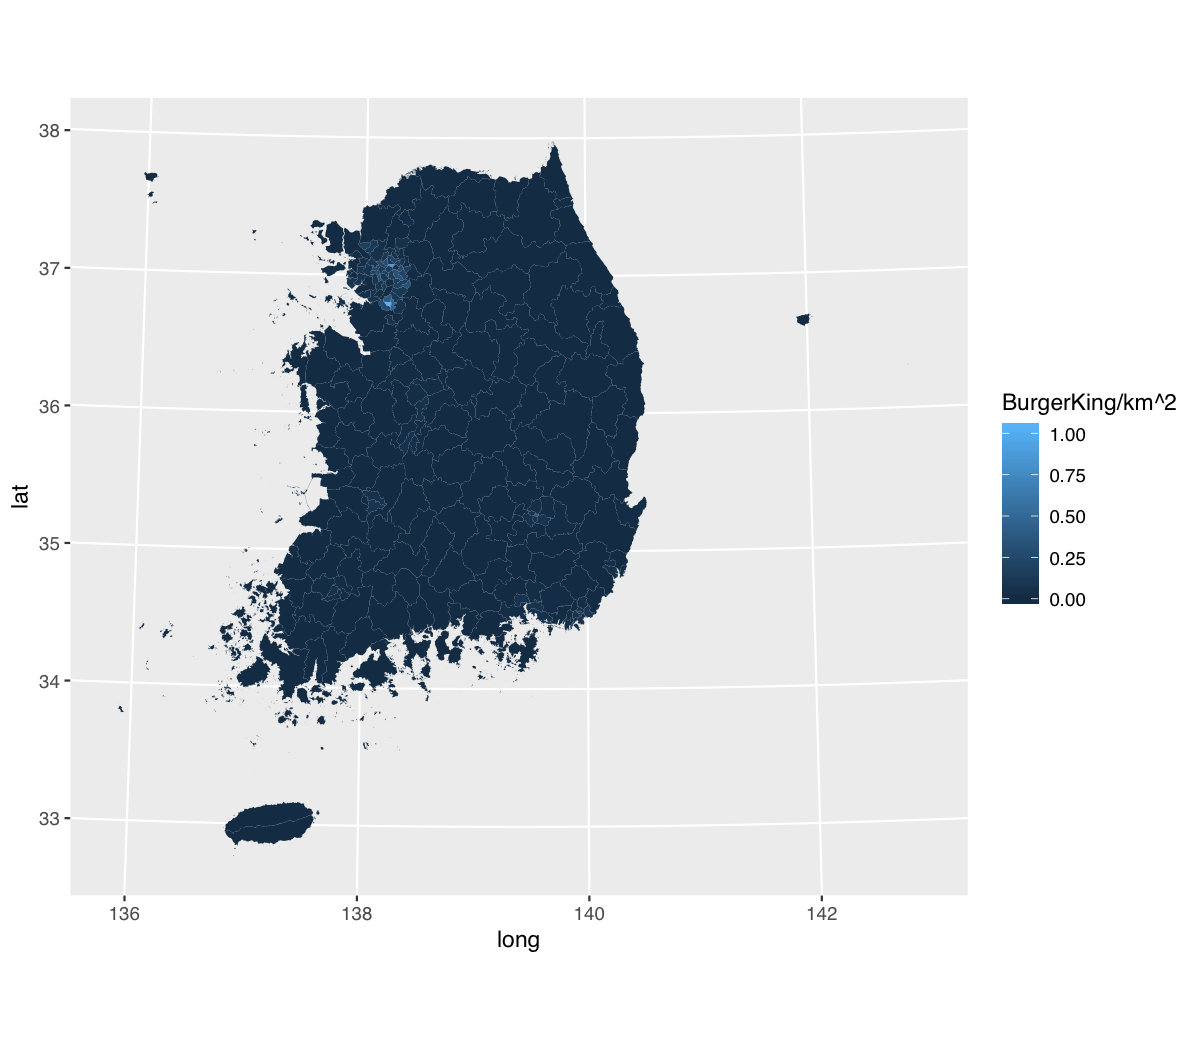
\includegraphics[width=\textwidth]{../figs/B_sig.png}
        \caption{버거킹}\label{fig:fastfood:B}
    \end{subfigure}
    \hfill
    \begin{subfigure}[b]{0.475\textwidth}  
        \centering 
        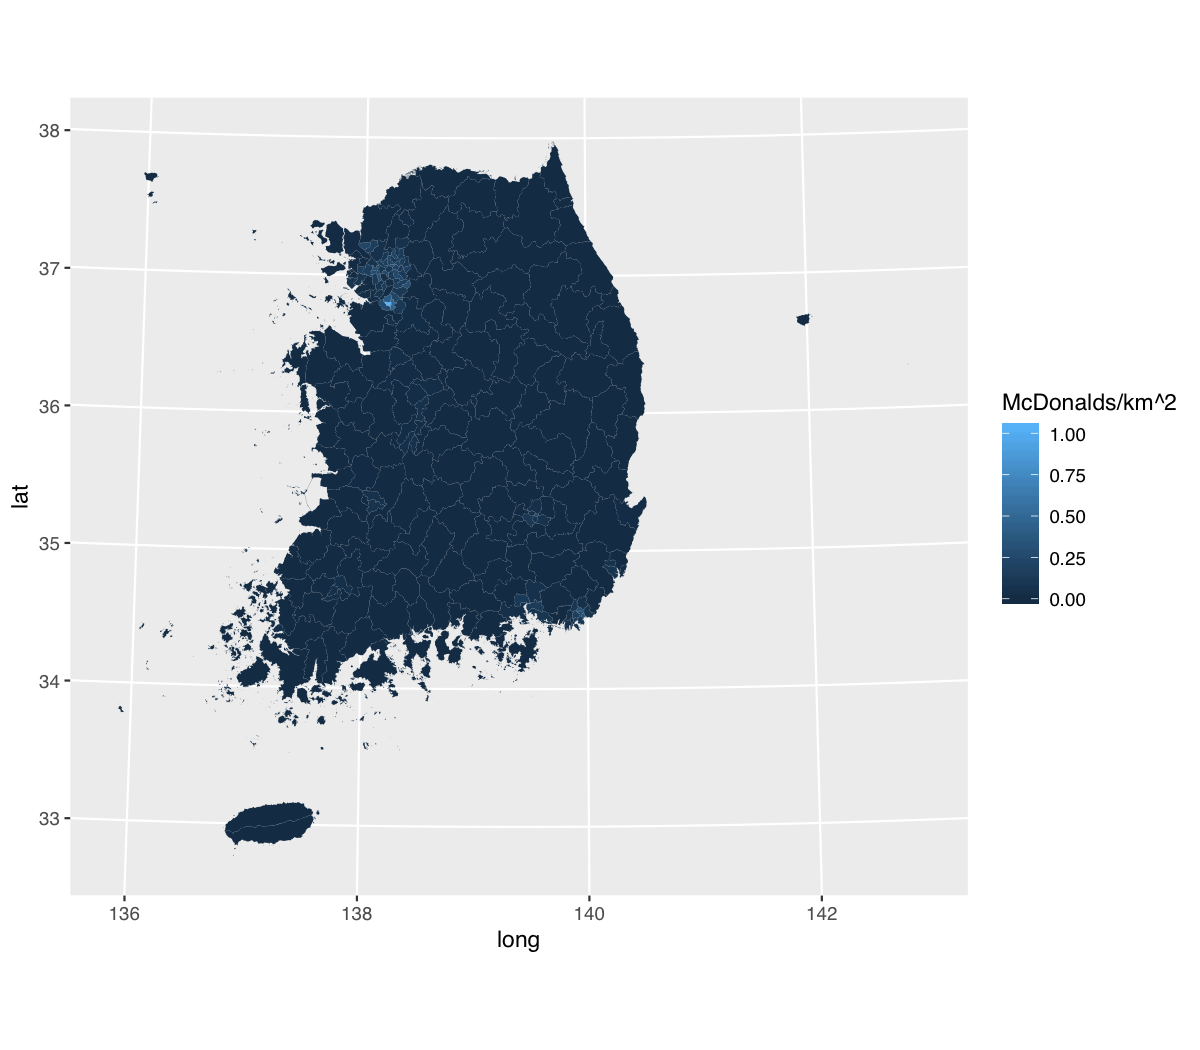
\includegraphics[width=\textwidth]{../figs/M_sig.png}
        \caption{맥도날드}\label{fig:fastfood:M}
    \end{subfigure}
    \vskip\baselineskip
    \begin{subfigure}[b]{0.475\textwidth}   
        \centering 
        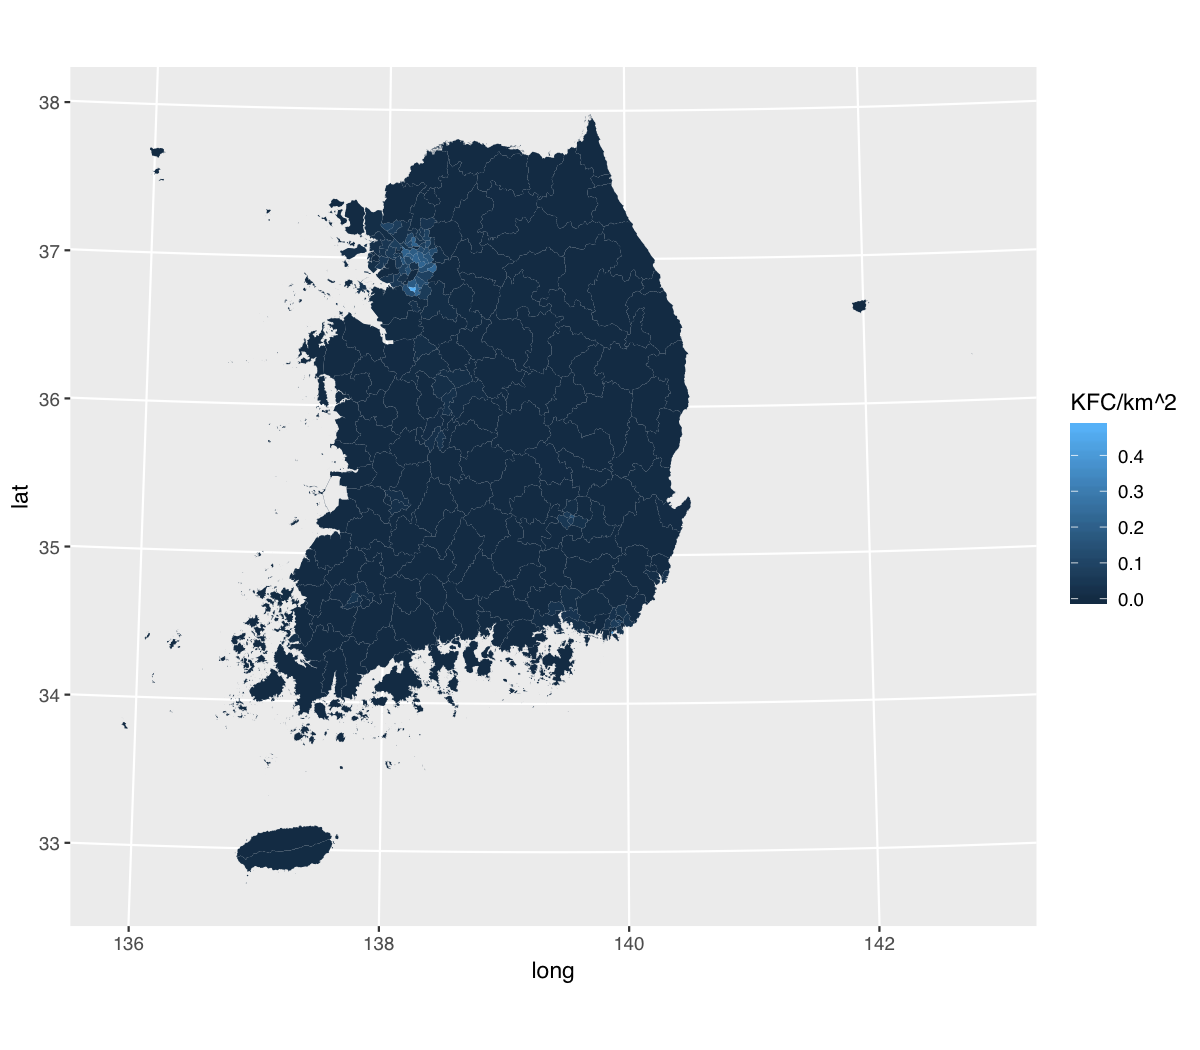
\includegraphics[width=\textwidth]{../figs/K_sig.png}
        \caption{KFC}\label{fig:fastfood:K}
    \end{subfigure}
    \quad
    \begin{subfigure}[b]{0.475\textwidth}   
        \centering 
        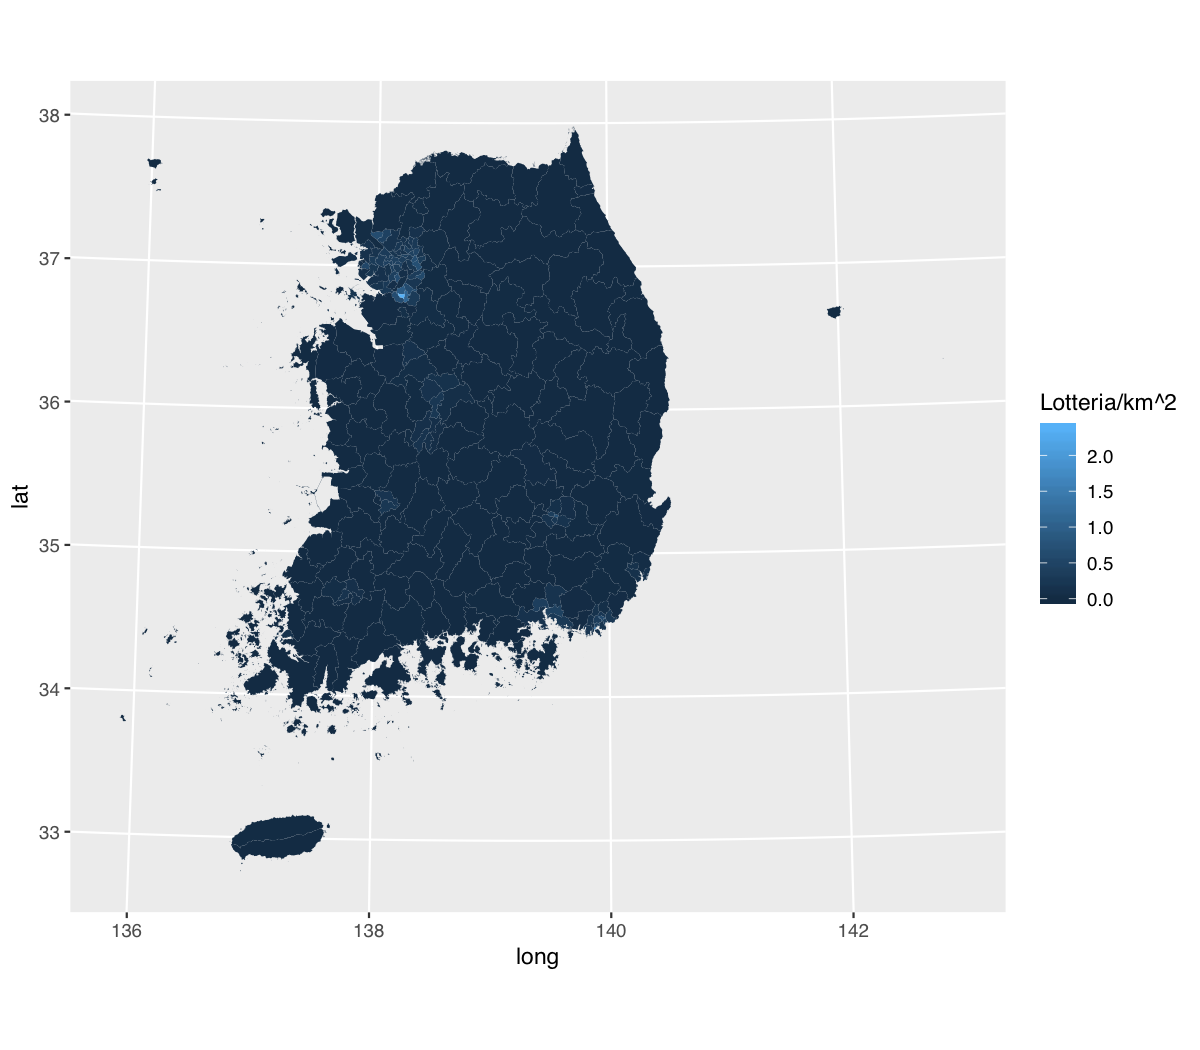
\includegraphics[width=\textwidth]{../figs/L_sig.png}
        \caption{롯데리아}\label{fig:fastfood:L}
    \end{subfigure}
    \caption{시군구별 제곱킬로미터당 패스트푸드 매장 수}
    \label{fig:fastfood}
\end{figure}   

\begin{figure}[!ht]
    \centering
    \begin{subfigure}[b]{0.475\textwidth}
        \centering
        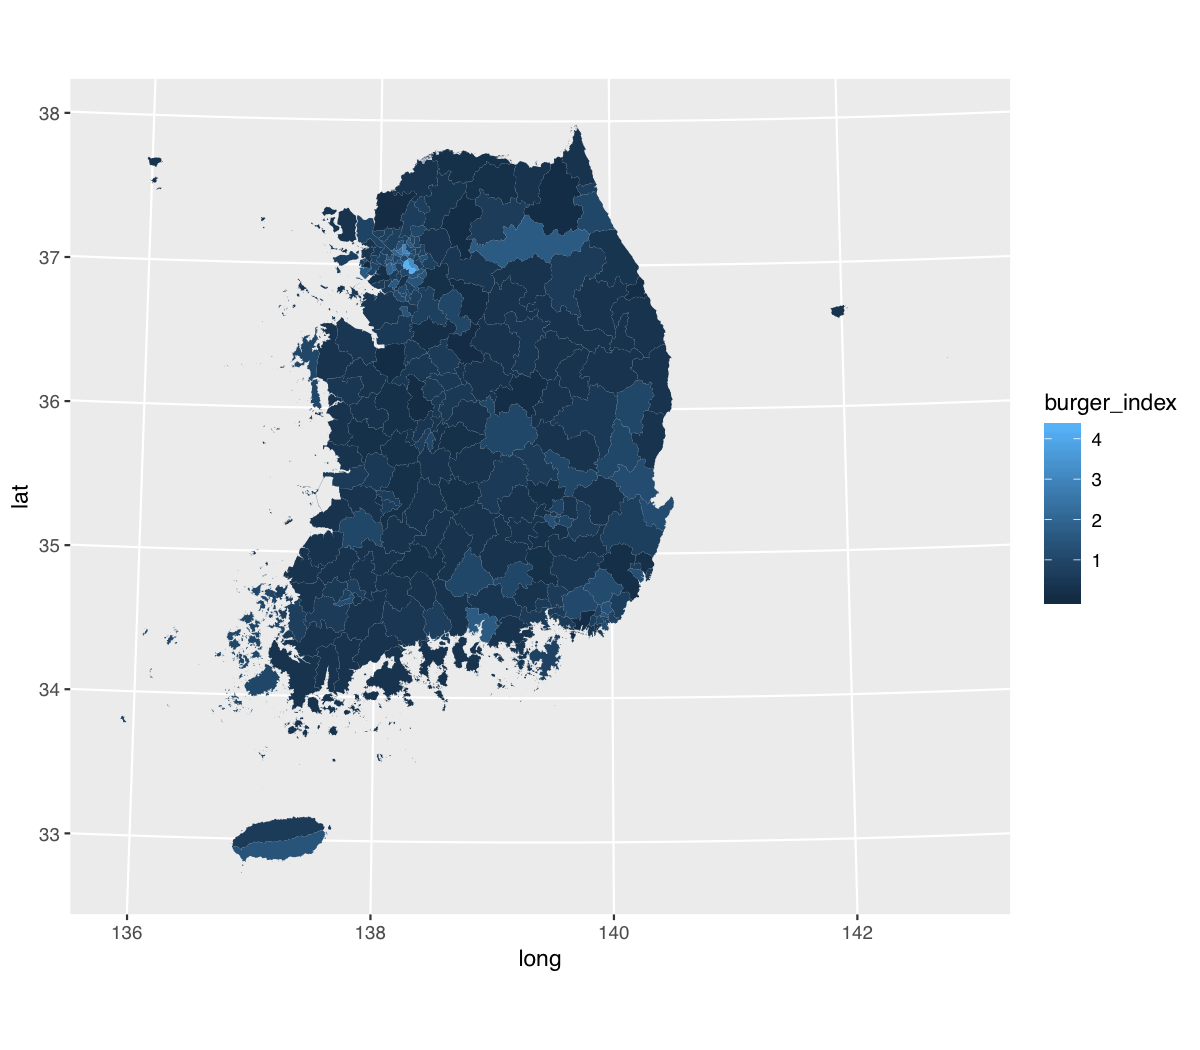
\includegraphics[width=\textwidth]{../figs/bi_sig.png}
        \caption{버거지수}\label{fig:bi}
    \end{subfigure}
    \hfill
    \begin{subfigure}[b]{0.475\textwidth}
        \centering
        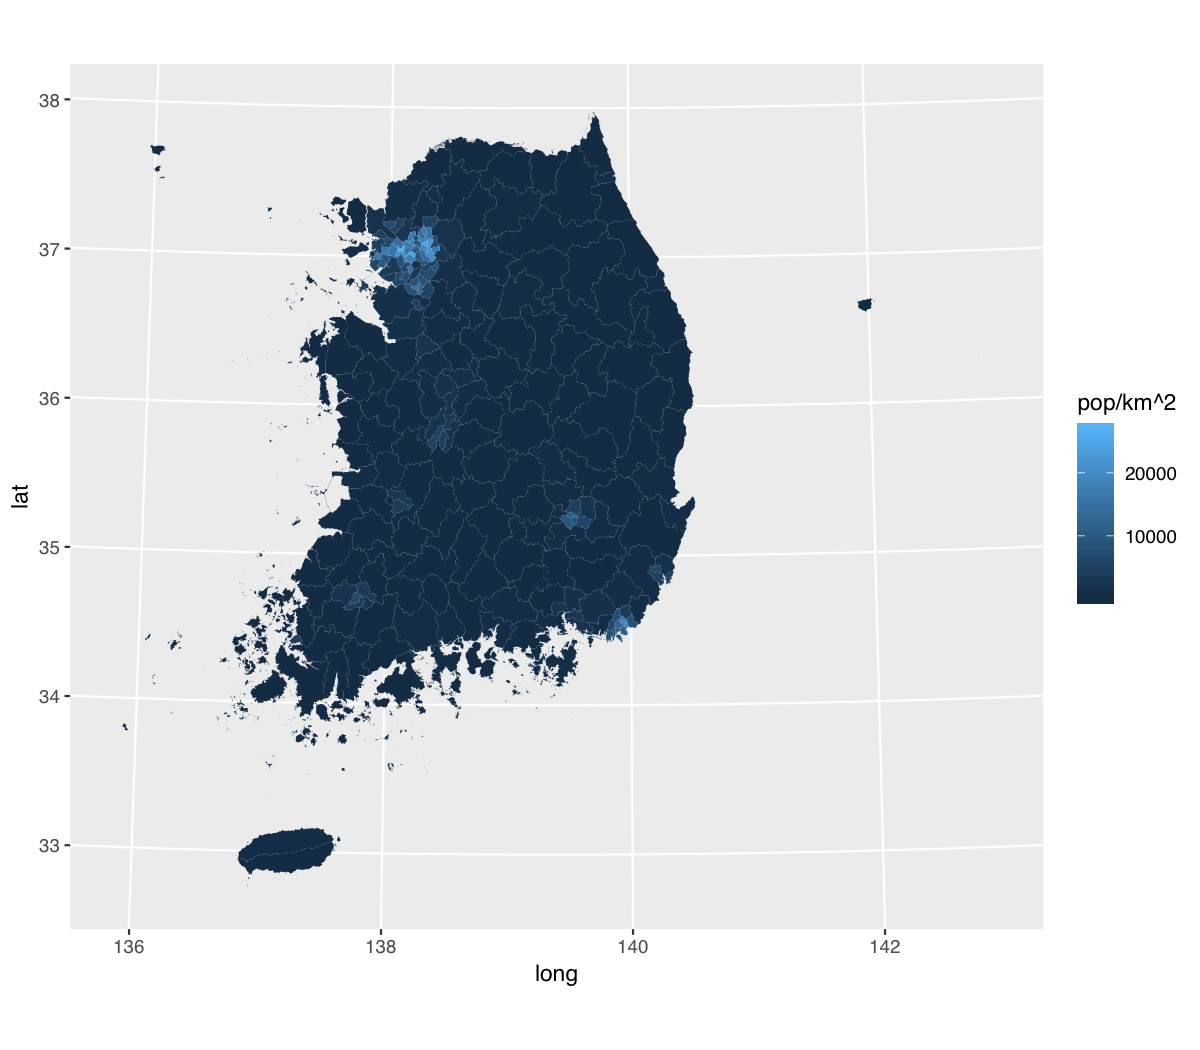
\includegraphics[width=\textwidth]{../figs/popden_sig.png}
        \caption{인구밀도}\label{fig:popden}
    \end{subfigure}
    \caption{버거지수와 인구밀도}\label{fig:biandpopden}
\end{figure}

\subsection{Numerical Analysis}\label{subsec:eda:numeric}

\autoref{tbl:summary}에 각 변수들의 요약통계량을 계산하였다. 앞서 예상한대로 롯데리아 매장 수가 다른 패스트푸드 브랜드에 비해 월등히 많다는 것과 지역별로 각 변수들의 표준편차가 매우 크다는 것을 확인할 수 있다. 분위수와 평균값을 확인해보면 자료의 분포가 왼쪽에 치우쳐져 있을 것이라 예상할 수 있다. 

\begin{table}[ht]
    \centering
    \begin{tabular}{c|rrrrrr}
      \hline
     & B & M & K & L & BI & pop\_density \\ 
     \hline
       mean & 1.94 & 2.26 & 1.11 & 7.48 & 0.68 & 4038.56 \\ 
       sd & 2.64 & 2.99 & 1.67 & 8.17 & 0.53 & 6083.81 \\ 
       Min. & 0.00 & 0.00 & 0.00 & 0.00 & 0.04 & 20.29 \\ 
       1st Qu. & 0.00 & 0.00 & 0.00 & 1.00 & 0.33 & 111.02 \\ 
       Median & 1.00 & 1.00 & 0.00 & 5.00 & 0.54 & 633.07 \\ 
       Mean & 1.94 & 2.26 & 1.11 & 7.48 & 0.68 & 4038.56 \\ 
       3rd Qu. & 3.00 & 4.00 & 2.00 & 10.00 & 0.90 & 6310.90 \\ 
       Max. & 13.00 & 13.00 & 10.00 & 34.00 & 4.27 & 27153.23 \\ 
    \hline
    \end{tabular}
    \caption{각 변수들의 요약통계량}\label{tbl:summary}
\end{table}

\autoref{fig:distribution}에 각 변수들의 분포를 나타내었다. 실제로 각 변수들은 왼쪽으로 치우쳐져 있으며 매장 수의 분포는 강한 양의 상관관계가 있다는 것을 확인할 수 있다. 또한, 버거지수와 인구밀도의 상관관계는 매장 수와 인구밀도의 상관관계보다 강한 것으로 확인된다. 
\begin{figure}
    \centering
    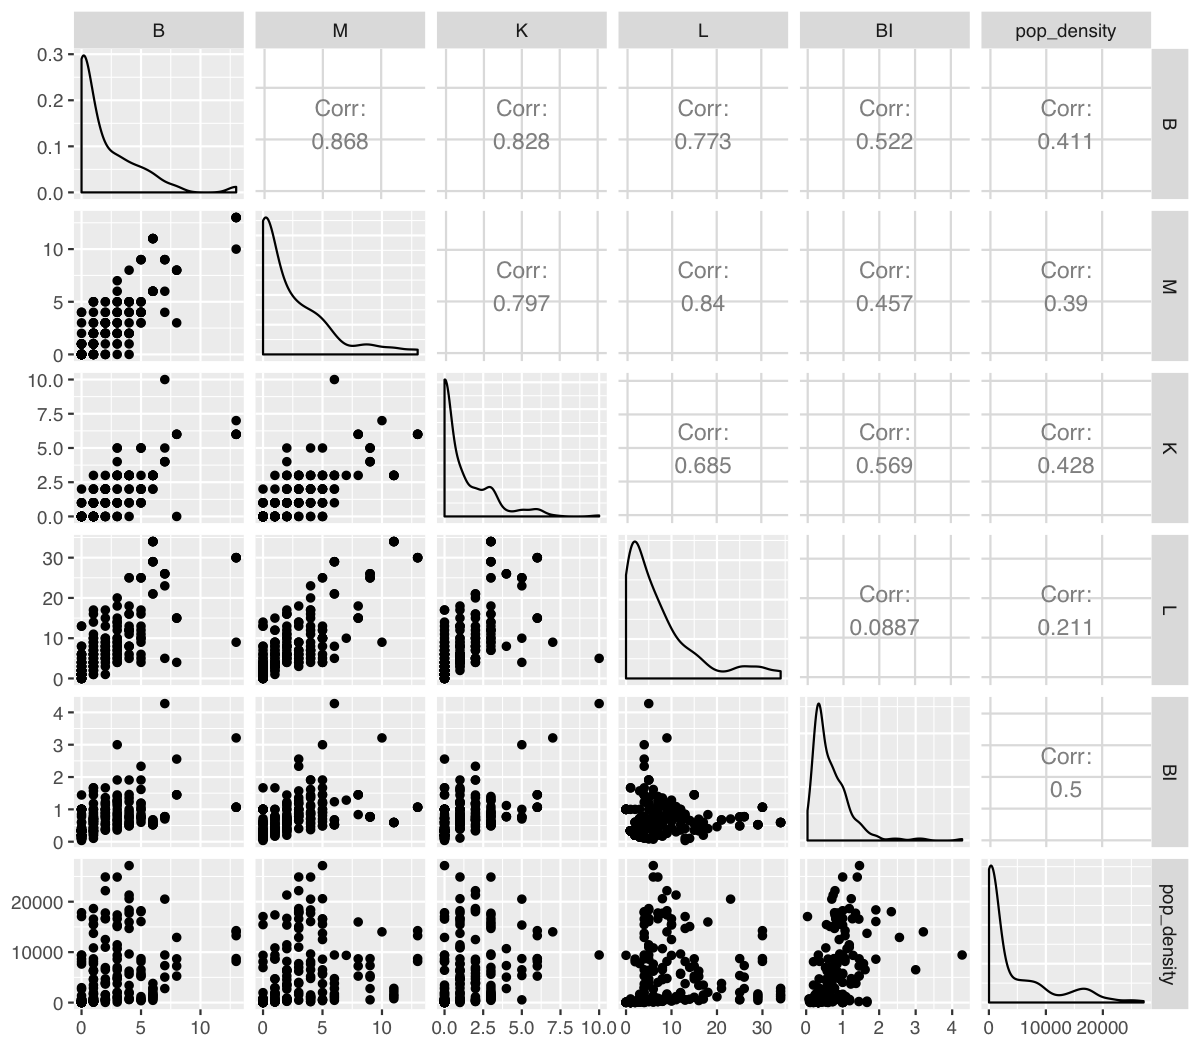
\includegraphics[width=0.7\textwidth]{../figs/dist_sig.png}
    \caption{각 변수들의 분포}\label{fig:distribution}
\end{figure}

\section{Spatial Regression Model}\label{sec:sreg}

\subsection{Model}\label{subsec:sreg:model}

본 보고서에서는 버거지수 $BI_i$가 다음과 같은 분포를 따른다고 가정하였다.


\section{Results}\label{sec:result}


\section{Conclusion}\label{sec:con}

본 보고서에서는 다각도로 버거지수를 분석하였다. GIS 자료를 이용해 버거지수를 시각화하였으며 도시 발전도와 상관관계가 있을 것이라 생각되는 인구밀도를 사용하여 공간회귀모형을 적합하였다. 시각화된 버거지수를 통해 기존의 위상구조를 이용한 시각화보다 훨씬 더 현실적인 형태의 분포를 확인할 수 있었으며, 회귀모형으로부터 인구밀도와 버거지수의 구체적인 관계를 확인할 수 있었다. 

향후 연구 방향으로 버거지수와 관련된 설명변수들을 제안하며 보고서를 마무리하고자 한다. 먼저, 도시의 생산량을 나타내는 도시별 GDP가 있다. 대한민국 통계청에서는 \href{http://kosis.kr/statHtml/statHtml.do?orgId=101&tblId=DT\_2KAA912\_OECD}{OECD 국가의 도시별 GDP}를 제공하고 있으나 시군구별 세분화된 자료를 얻을 수 없어 이번 분석에서는 제외하였다. 이 외에도 도시의 생산량에 영향을 미치는 생산가능인구 비율, 산업 구조 등을 설명변수로 사용한다면 보다 현실적인 모형을 적합할 수 있을 것이라 기대한다.

\bibliography{refs}

\end{document}